%%This is a very basic article template.
%%There is just one section and two subsections.
\documentclass{article}
\usepackage[a4paper, margin=2.5cm]{geometry}
\usepackage{amsmath}
\usepackage{mathtools}
\usepackage{amssymb}
\usepackage{caption}
\usepackage{placeins}
\usepackage{graphicx}
\usepackage{subcaption}
\usepackage{setspace}
\usepackage{float}
\usepackage{wrapfig}
\usepackage{pdfpages}
%\usepackage[active,tightpage]{preview}
\usepackage{natbib}
\bibpunct{(}{)}{,}{a}{}{;} 
\usepackage{url}
\usepackage{nth}
\usepackage{authblk}
\usepackage{blindtext}
\usepackage{makecell}
\usepackage{endnotes}

\let\footnote=\endnote
%\usepackage{fontawesome}
% \renewcommand\theadalign{bc}
% \renewcommand\theadfont{\bfseries}
% \renewcommand\theadgape{\Gape[4pt]}
% \renewcommand\cellgape{\Gape[4pt]}
\DeclarePairedDelimiter\floor{\lfloor}{\rfloor}
% for the d in integrals
\newcommand{\dd}{\; \mathrm{d}}
\newcommand{\tc}{\quad\quad\text{,}}
\newcommand{\tp}{\quad\quad\text{.}}
\newcommand{\ra}{\rightarrow}
\def\lsub#1#2%
  {\mathop{}%
   \mathopen{\vphantom{#2}}_{#1}%
   \kern-\scriptspace%
   #2}
\def\lsup#1#2%
  {\mathop{}%
   \mathopen{\vphantom{#2}}^{#1}%
   \kern-\scriptspace%
   #2}

\defcitealias{HMD}{HMD}
\defcitealias{HFD}{HFD}
\newcommand\ackn[1]{%
  \begingroup
  \renewcommand\thefootnote{}\footnote{#1}%
  \addtocounter{footnote}{-1}%
  \endgroup
}
\newcommand\todo[1]{\textcolor{red}{[TODO: #1]}}
\newcommand\high[1]{\colorbox{yellow}{#1}}
\begin{document}

%  Research note, up to 3,500 words.
% presently ca 2400 not including appendix.
% \title{Boom, echo, pulse, flow}
% \author[1]{Tim Riffe\thanks{riffe@demogr.mpg.de}}
% \author[1]{Kieron Barclay}
% \author[1]{Christina Bohk-Ewald}
% \author[2]{Sebastian Kl\"usener}
% \affil[1]{Max Planck Institute for Demographic Research}
% \affil[2]{Federal Institute for Population Research}
% \maketitle
(Submitted as Research Note)
\paragraph{Title} Boom, Echo, Pulse, Flow: 385 Years of Swedish Births
\paragraph{Short title} Boom, Echo, Pulse, Flow
\paragraph{Authors} Tim Riffe*, Kieron Barclay, Sebastian Kl\"usener, Christina Bohk-Ewald
\paragraph{(*)} Corresponding: Tim Riffe \texttt{riffe@demogr.mpg.de}

\paragraph{Author information} ~
\begin{table}[ht]
\begin{center}
\begin{tabular}{llll}
Name & Affiliation & ORCID & \includegraphics[height=1em]{Figures/twitter.png}  \\ \hline
T. Riffe & Max-Planck-Institute for Demographic Research & 0000-0002-2673-4622 & \texttt{@timriffe}  \\
K. Barclay & Max-Planck-Institute for Demographic Research &  & \texttt{@BarclayKieron}  \\
S. Kl\"usener &Federal Institute for Population Research& 0000-0003-0436-3565 & \texttt{@demomapper}  \\
C. Bohk-Ewald & Max-Planck-Institute for Demographic Research &  &
\end{tabular}
\end{center}
\end{table}

\paragraph{Disclosure statement} We have no conflicts of interest with any aspect of this work. 

\paragraph{Data availability statement} All data and \texttt{R} code required to reproduce this work in its entirety is available in a \texttt{github} repository: \texttt{https://github.com/timriffe/BirthFlows}. This may be placed in an Open Science Framework repository later on.

\paragraph{Supplemental online material} We propose to locate the appendices in supplementary online material, since they are 1/2 of the manuscript. Per correspondence with the editors prior to submission, the very large Fig.~\ref{fig:foldout} will likely need to go at the end of the print article rather than where it is indicated in the text. In this case we would change the text to make sure it is referred to appropriately. We propose to offer a redundant copy of this figure in the supplementary online material as well.}

\doublespacing
\pagebreak
% presently ca 2400 not including appendix.
\title{Boom, echo, pulse, flow: 385 years of Swedish births}
 \author{Author(s) redacted}
% \author[1]{Kieron Barclay}
% \author[1]{Christina Bohk-Ewald}
% \author[2]{Sebastian Kl\"usener}
% \affil[1]{Max Planck Institute for Demographic Research}
% \affil[2]{Federal Institute for Population Research}
\maketitle

\pagebreak
\begin{abstract}
Human population renewal starts with births. Since births can happen at any
time in the year and over a wide range of ages, demographers typically imagine
the birth series as a continuous flow. Taking this construct literally, we
visualize the Swedish birth series as a flow. A long birth series allows us to
juxtapose the children born in a particular year with the children that
they in turn had over the course of their lives, yielding a crude notion of
cohort replacement. Macro patterns in generational growth define the meandering
path of the flow, while temporal booms and busts echo through the flow with the
regularity of a pulse.
\vspace{1em}

{\bf Keywords:} Fertility, Population structure, Population momentum, Population renewal, Data visualization
\end{abstract}

\pagebreak
\section{Introduction}
Usually demographers think of fertility as an age-regulated process. In any case it is bounded by menarche and menopause, both of which are anchored to biological age. These anchors may move, but not far or fast. And between these bounds, at least within acceptably homogeneous subpopulations, fertility patterns appear to conform to some regular schema. Since births can happen at any time throughout the year and throughout the fertile age range, and since demography usually deals in large numbers, it is common to imagine births at the population level as a continuous stream or flow. This is so not only as a pragmatic assumption to allow for calculus, but it also gives us a heuristic understanding of fertility as a smoother of population structure \citep{arthur1982ergodic}. In the present exposition, we retreat from rates, the basis of projections and stable theory, to the absolute number of babies born, the raw material of population renewal. 

We aim to represent a long time series of birth counts as a multilayered view of population renewal, a perspective enabled by Sweden's long history of population statistics. The birth series is rendered as a flow, in such a way as to simultaneously suggest several analytic perspectives, and to invite newcomers and curious minds deeper into the discipline of demography. This image, a large fold-out insert, entails investment from the viewer, and this manuscript serves as a protracted legend and caption. It is not a concise analytic plot, but rather a composite of hundreds of distributions, rendered both in the period and cohort perspectives. Intellectual payoffs include a simultaneous sense of long term patterns of generational mixing and generational replacement, medium term baby booms and echos, and the short term shocks of population momentum. %We challenge more experienced demographers to relate this image to the Lexis diagram, to imagine how the picture would change if fertility were indexed to fathers' age, or to reimagine this image of aggregates as an immense set of lineages.

Our Lexis time series of birth counts stretches from 1735 until 2016, and it is augmented by a projection of the completed fertility of cohorts through 2016, bringing the latest year of birth to 2071. The temporal spread from the earliest mother cohort in our final data set (1687) to the latest offspring cohort (2071) is 385 years. We describe our input data and adjustments to it briefly in Sec..~\ref{sec:data}, and in a detailed set of appendices. Sec.~\ref{sec:birthdist} relates different age-structured birth count distributions to a common calendar. These distributions become the basic elements of our visualization. Sec.~\ref{sec:description} gives a plain language description of how to interpret the visualization and a guide through some of its major features. Sec.~\ref{sec:disc} discusses the strengths and limitations of this particular visualization, and Sec.~\ref{sec:conc} concludes with a summary of this work.

\section{Data and methods}
\label{sec:data}
We would like for our visualization to be an exposition on human renewal in general, but this work will be most useful if based on a long data series of good quality, ergo a single population with its own history and peculiarities. As \citet{perozzo1880della}, we base our exposition on Sweden because the data are available and of adequate dimension, but there are two ways in which this fact is not to be taken for granted: i) The data comes from multiple sources and formats, it varies in quality, and it must be brought to a common Lexis resolution to be useful, and ii) although the visualization shows a history of birth in Sweden in particular, it may serve as a parable for multiple demographic models of a general nature.

The visualization is based on birth count data from Sweden in single-year bins by year of occurrence (period) and mother cohort. Birth counts for years 1736 to 1750 are reconstructed from a variety of sources \citep{HFC, HMD, sweden1969historisk} using indirect methods (see App.~\ref{app:retroject}). Data for years 1751-1774 are derived via adjustment from HFC estimates and HMD exposures and birth totals (see App.~\ref{sec:hfc}). Data for the period 1775 to 1890 come from \citet{sgf1907}, which we have graduated from mostly five-year age groups into single ages (see App.~\ref{sec:sgf}). The merged birth count series for years 1736 to 1890 is subject to a global adjustment to retain information on cohort size in period birth distributions (see App.~\ref{sec:histadj}). Data for the years 1891 to 2016 is taken directly from the \citet{HFD} without further adjustment, although the HFD itself did split single age birth counts into Lexis triangles from years 1891 to 1869 \citep{persson2010human}. To complete our picture, we project the fertility of cohorts whose fertility careers were still incomplete as of 2016 (1962-2016) through age 55 (see App.~\ref{sec:proj}). These steps are fully reproducible, and further details can be found in an open data and code repository.

\section{Birth count distributions in period and cohort perspectives}
\label{sec:birthdist}

The main fold-out visualization we present (Fig.~\ref{fig:foldout}) is a composition of smaller elements, each a birth distribution. We therefore build up to its full description by making explicit some basic notions of birth distributions and the calendar time line, drawing a distinction between two kinds of birth distributions featured in the final plot. This is intended to aid in the interpretation of the main figure. 

In the period perspective, a picture of the births is for demographers most instinctively broken down by the age of mothers who gave birth in that year, Fig.~\ref{fig:agemother}, or by the year of birth of mothers Fig.~\ref{fig:cohmother}. These two distributions are essentially identical, but appear as mirror images if chronological time is enforced in $x$. This is key: In the period perspective with births arranged on an age axis, young mothers are on the left and older mothers on the right, but the reverse is true on a cohort axis. Count distributions such as this may be jagged, even if the underlying rate distributions are smooth, due to population structure.\footnote{The deficit around age 31 in \ref{fig:agemother} is due to a smaller number of potential mothers: Cohorts born between 1867 and 1869 were smaller than the surrounding cohorts due to a famine in those years.} 

\begin{figure}[ht!]
\begin{subfigure}[t]{0.5\textwidth}
        \centering
        \includegraphics[width=\textwidth]{Figures/Fig11900MotherAge.pdf}
        \caption{Births in 1900 by age of mother}
        \label{fig:agemother}
\end{subfigure}
~
\begin{subfigure}[t]{0.5\textwidth}
        \centering
        \includegraphics[width=\textwidth]{Figures/Fig11900MotherCohort.pdf}
        \caption{Births in 1900 by year of birth of mother}
          \label{fig:cohmother}
\end{subfigure}
\caption{Births in a year structured by mothers' age versus mothers' year of birth are a
reflection over $y$ and shift over $x$. }
\end{figure}

Given a long-enough time series of births classified by age and/or mother cohort, the full reproductive career of the cohort of individuals born in a particular year can be represented as a distribution (assuming no effects of migration). Since the childbearing of a cohort is spread over a synchronous span of ages and years, the $x$-indexing by age (Fig.~\ref{fig:age1900mother}) or year (Fig.~\ref{fig:year1900}) yields identical and redundant distributions: there is no reflection of young and old mothers when toggling between age and period classifications in the cohort perspective: In both cases young mothers are on the left and older mothers on the right. The distribution of births over the lifecourse of a cohort often resembles the smoothness of fertility rate schedules, but this is not necessarily the case.

\begin{figure}[ht!]
\begin{subfigure}[t]{0.5\textwidth}
        \centering
        \includegraphics[width=\textwidth]{Figures/Fig11900IDAge.pdf}
        \caption{Births from mothers born in 1900 by age of mother}
        \label{fig:age1900mother}
\end{subfigure}
~
\begin{subfigure}[t]{0.5\textwidth}
        \centering
        \includegraphics[width=\textwidth]{Figures/Fig11900IDYear.pdf}
        \caption{Births from mothers born in 1900 by year}
          \label{fig:year1900}
\end{subfigure}
\caption{Births of a cohort structured by mothers' age versus mothers' year of birth are a shift over $x$. }
\end{figure}

The births in a year are classified by mothers' cohort, i.e. cohort \emph{origins} in Fig.~\ref{fig:cohmother}, whereas the births \emph{from} a cohort are classified \emph{to} period in Fig.~\ref{fig:year1900}. The two distributions are different in kind, but relatable and both on a common scale. Importantly, these two distributions are indexed to the same calendar line. A fuller representation of their relationship would place them as two disjoint distributions on the same timeline, as in Fig~\ref{fig:juxt}.

\begin{figure}[ht!]
 \centering
        \includegraphics[width=\textwidth]{Figures/Fig31900juxt.pdf}
        \caption{The cohort distribution of mothers who gave birth in 1900 (\textbf{A}) and the births from mothers born in 1900 by year (\textbf{B}). These two distributions imply \emph{three} generations: the mothers of the 1900 cohort, the cohort of 1900 itself, and the offspring of the 1900 cohort.}
          \label{fig:juxt}
\end{figure}

The two distributions on the calendar axis in Fig.~\ref{fig:juxt} are related, and of comparable scale, but different in kind. The $x$ coordinate of the left distribution \textbf{A} is indexed to mothers' birth cohort (old to young), whereas the $x$ coordinate of the right distribution \textbf{B} is indexed to child cohort, occurrence year (young to old). In this way the respective $x$ coordinates are two generations apart, relating to each other as grandmothers and grandchildren. These are two distributions that we may wish to compare in various ways to better understand the birth series, but doing so for the entire Swedish dataset presents a practical challenge for a single visualization. 

For the case of our extended Swedish birth series, we have 281 distribution pairs such as the year 1900 dual shown in Fig.~\ref{fig:juxt}, making simultaneous rendering impractical unless we transform the data in some way. An honest attempt might look like Fig.~\ref{fig:reflect1}, where we reflect the left distribution \textbf{A} over $y$, keeping \textbf{B} on the top axis. These two distributions are linked by the year 1900, the reference year, which of course overlaps with neither of them. In this representation, distributions \textbf{A} and \textbf{B} are re-drawn for each possible reference year from 1736 to 2016, and therefore imply a large sequential set of overlapping distributions. Each \nth{20} distribution is highlighted, but despite attempts to make this graph legible, i) the high degree of overlapping and ii) the spatial dissociation of each \textbf{A} --- \textbf{B} pair makes the intended comparison difficult over the series. These two drawbacks hide some macro patterns present in the data.

\begin{figure}[ht!]
 \centering
        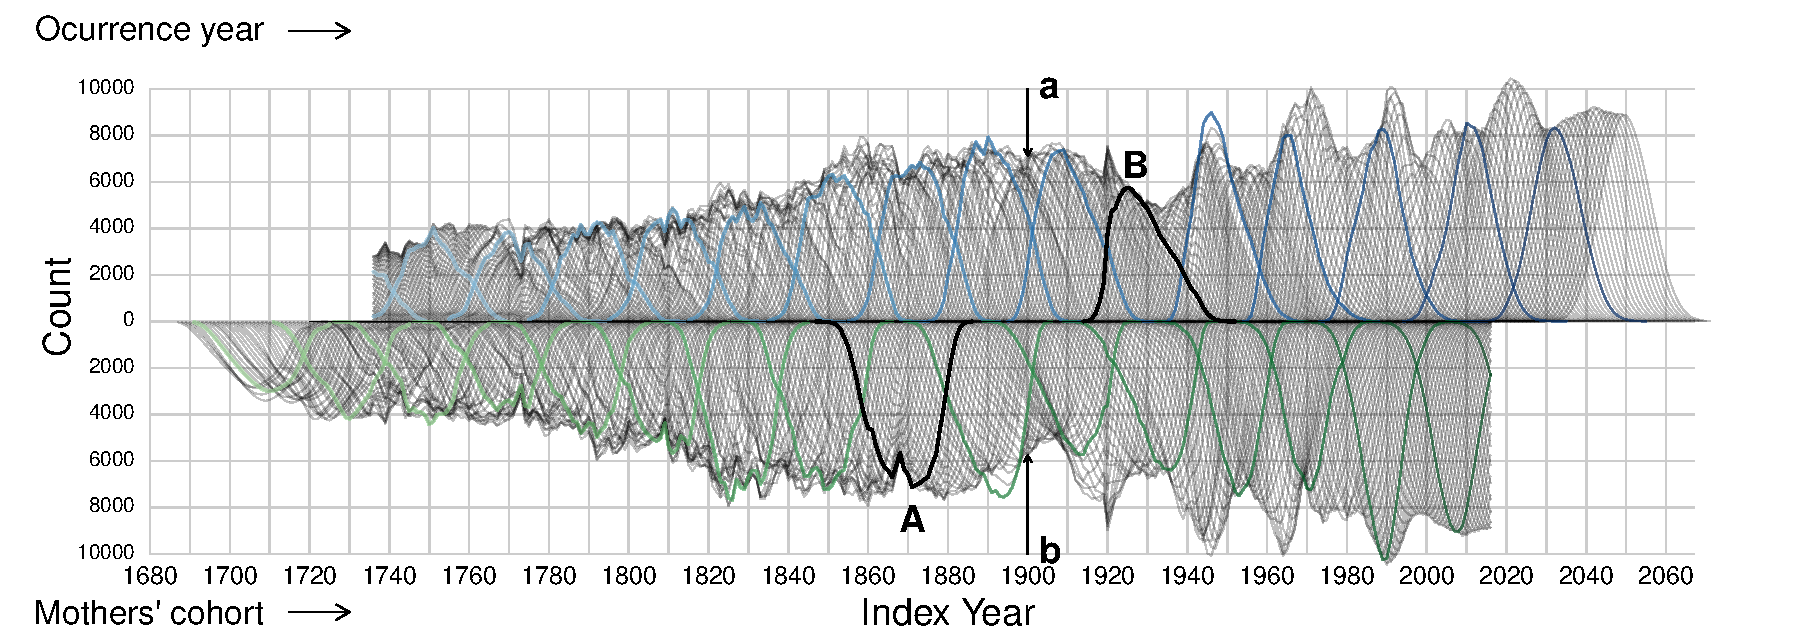
\includegraphics[width=\textwidth]{Figures/FxFlowReflect.pdf}
        \caption{One time series of birth count distributions, under the period and cohort perspectives. The top series is composed of cohort offspring distributions indexed to period. The bottom series is composed of period birth distributions indexed to mothers' cohort. \textbf{A} and \textbf{B} are the same as in Fig.~\ref{fig:juxt}. The cross-section \textbf{a} gives \textbf{A} and the cross-section \textbf{b} gives \textbf{B}.}
          \label{fig:reflect1}
\end{figure}

Still, the reflected axes Fig.~\ref{fig:reflect1} produce at least two noteworthy artifacts that we may wish to preserve and clarify: i) First order differences in the top series appear to cascade into the lower series--- This highlights a small constituent of population momentum \citep{keyfitz1971momentum}: larger cohorts tend to have more offspring than smaller neighboring cohorts and vice versa, sudden fertility rate changes notwithstanding. ii) The composition of \textbf{A} in the bottom series is implied by the cross-section \textbf{a} of the top series, and the composition of \textbf{B} is implied by the cross-section \textbf{b}. This second observation merits further elaboration: Since we have re-plotted the same series twice, each birth and each distribution is present in the plot twice. \textbf{A} and \textbf{B}, the two distributions we would like to juxtapose in bulk, are found indexed to the same reference year in the cross sections \textbf{a} and \textbf{b}. Alignment on a single reference year ought to facilitate comparison, but this visual task is stymied because the points constituting cross-sections \textbf{a} and \textbf{b} are heavily overlapped. 

\pagebreak
% text above pushes whole thing down
\begin{wrapfigure}{r}{0.5\textwidth}
 \centering
        \includegraphics[width=3in]{Figures/FigReflection.pdf}
        \caption{The 1900 cohort as a composite bar with its offspring reflected over $y$. The size of each bar stacked in the top composition is proportional to the area of its corresponding polygon in the left distribution \textbf{A} of Fig.~\ref{fig:juxt}. The size of each bar stacked in the lower composition is proportional to the area of its corresponding polygon in the right distribution \textbf{B} of Fig.~\ref{fig:juxt}. This is the same as stacking the slices of \textbf{a} and \textbf{b} from Fig.~\ref{fig:reflect1} }
          \label{fig:refl}
\end{wrapfigure}
% text under goes to the left then builds down
If instead we stack the slices that are indecipherably overlapped in \textbf{a} and \textbf{b} we get something like that shown in Fig.~\ref{fig:refl}, cumulative birth distributions. %Young mothers are on top and older mothers on bottom for both distributions. It would also make sense to plot increasing (or decreasing) ages emanating out from the centerline in both directions. 
Here the total bar length is proportional to the total cohort size of \textbf{a} and total offspring size of \textbf{b}. Stacked bins reflect 5-year mother cohorts in \textbf{a} and 5-year periods in \textbf{b}. From this representation it is clear that mothers born in the 20 years between 1860 and 1880 produced the bulk of the 1900 cohort (86\%), which itself produced the majority of its offspring in the 20 years between 1920 and 1940 (90\%). It is also quite visible that the 1900 cohort did not replace itself in a crude sense: 138,139 babies formed a cohort whose eventual mothers gave birth to 95,379 babies over the course of their lives, a crude replacement of 69\%. Other perspectives on reproduction that account for survival and attrition or growth of the mother cohort through migration would give a more optimistic assessment of reproductivity \citep{henry1965reflexions}, a subject we return to in the discussion. The key feature of Fig.~\ref{fig:refl} is that the two distributions that are disjoint when drawn on a calendar line in Fig.~\ref{fig:juxt}, and that are hard to pick out in Fig.~\ref{fig:reflect1} can now be associated at a common $x$ coordinate, and with distinguishable bins. This transformation allows us to view the time series of Fig.~\ref{fig:reflect1} with greater clarity, and it is the plot element from which our main Fig.~\ref{fig:foldout} is composed. 

If we repeat the exercise of Fig.~\ref{fig:refl} for each reference year in our data, and then merge neighboring like-bounded bins, we get something like Fig.~\ref{fig:joinbins}. This is just the same as taking the distributions of Fig.~\ref{fig:reflect1}, grouping in quinequennial bins, and then stacking them instead of overlapping them. That is, the filled polygons on the top axis represent the births of mothers from quinquennial cohorts, spread over occurrence years. On the bottom axis, filled polygons show the births in quinquennial periods indexed in $x$ to mothers' cohort. This is the skeleton of our main visualization.

\begin{figure}[ht!]
 \centering
        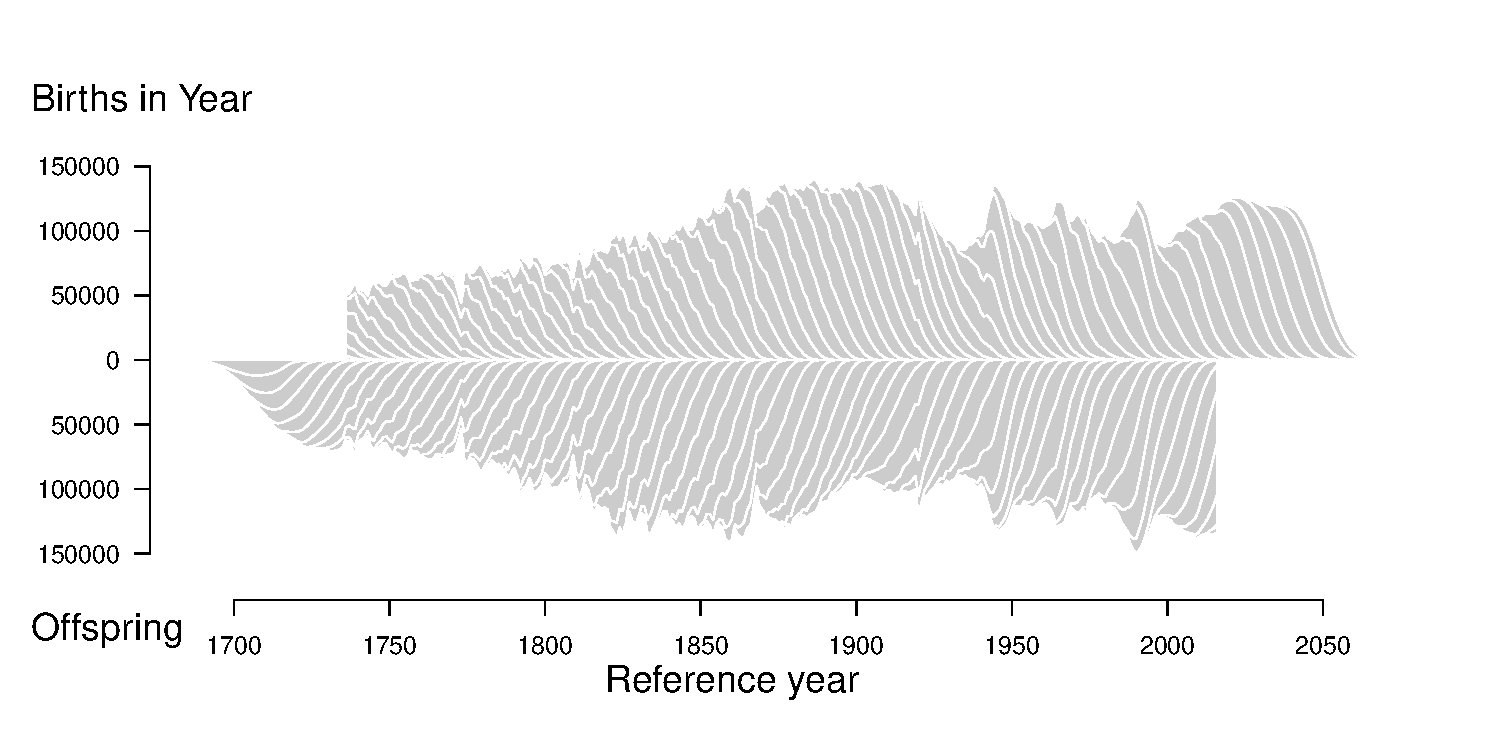
\includegraphics[width=\textwidth]{Figures/JoinBins.pdf}
        \caption{One time series of birth count distributions, under the period and cohort perspectives. The top series is composed of stacked polygons representing the quinquennial mother cohort birth distributions indexed to period. The bottom series is composed of stacked polygons representing quinquennial period birth distributions indexed to mothers' cohort. This is the underlying structure of fold-out Fig.~\ref{fig:foldout}.}
          \label{fig:joinbins}
\end{figure}

\section{A guide to the visualization.}
\label{sec:description}
This section serves as a guide to interpreting our primary visualization (fold-out Fig.~\ref{fig:foldout}). We first describe the primary visual attributes so that the reader may seek meaning in patterns, and we then narrate some of the more salient features of the graph.

\paragraph{Meandering baseline} We start with the stacked polygon representation in Fig.~\ref{fig:joinbins}, and subject it to a single $y$ transformation before re-plotting in our primary figure. This transformation is a $y$ shift proportional to a smoothed time series of the crude cohort replacement ratio (see App.~\ref{sec:baseline} for details), which in effect creates a meandering baseline rather than a flat $x$-axis. We call this crude replacement because the ratio takes no account of mortality or migration. TA horizontal white line crosses the middle region of the plot showing where the baseline would have to be to indicate exact crude replacement. Regions where the baseline is above the horizontal cut point, such as the first half of the \nth{19} century, are cohorts that produced a crude surplus of offspring, and vice versa. This transformation distorts the series somewhat, but we think in such a way as to make long term macro patterns more visible rather than to blend them out.

\paragraph{Profile} The height of each series vis-\`a-vis the baseline represents the total births in each year on the top series and the total births that each cohort had on the bottom series (the children they had). Due to the meandering baseline, long term trends must be sought out with some effort by comparing the profile with the nearest meandering $y$ grid line. This is not the kind of variation that the visualization focuses on. We consider short and medium term fluctuations to be of greater interest in this visualization. The pattern of single-year matched fluctuations in cohort and offspring size is retained, as is the matched sinusoidal pattern of medium term booms and busts in the \nth{20} century.

\paragraph{Stacked distributions} Shaded areas depict two kinds of birth distributions. On the top axis, each polygon is the offspring of a quinquennial cohort, indexed to the calendar years in which the births ocurred. Each distribution runs from left to right, stacked atop the previous cohort distribution. Therefore, births of young mothers are those closest to the outer profile, and births of older mothers approach the baseline. On the bottom axis, each polygon is the distribution of births in a quinquennial period, back-indexed to the mother cohort $x$ position on the calendar. Each distribution runs from older mothers on the left (outer profile) to younger mothers on the right (approaching baseline). 

\paragraph{Shading color}
Each polygon stacked in this visualization represents a birth distribution. We would like to highlight some characteristic of these distributions that may enhance our ability to detect patterns in this series. We opt to color based on the spread of each distribution, as defined by the birth-weighted standard deviation of maternal age at birth. The top and bottom shade colors are drawn from the same colorblind-friendly palette \citep{viridis}, where light colors mark wider distributions and dark colors mark relatively compact distributions. Underlying values range from 4.9 to 6.7 for period distributions (bottom) and from 5.1 to 6.7 for cohort distributions (top). There is a clear shift from wider to narrower distributions for cohorts born after around 1910 and occurrence years after about 1960.

\paragraph{Lineage}
To aid the viewer with interpretation, we overlay a five-generation maternal lineage, which includes Alva Myrdal (born Reimer), who as much as anyone ought to remind us of the endogenous forces in the birth series we depict.\footnote{Alva Myrdal designed policies to make childbearing more compatible with womens' work, to improve child wellbeing, and she was instrumental in other aspects of the Swedish welfare state. She also received a Nobel Peace Prize in 1982 for her work with the United Nations on disarmament, and for her influential writings on the topic of disarmament.} Since the top and bottom portions of the graph are alternative depictions of the same data, each member of this lineage appears twice: once below her mother at the same $x$ position, and once again on the top axis $x$-indexed to the year of birth and $y$ indexed to mother cohort. 

Anna Lisa was born in 1829, destined to become Alva's great grandmother. Anna Lisa gave birth to Anna Sofia in 1856. Anna Sofia therefore belongs to the offspring of the 1829 cohort, appearing directly below Anna Lisa and inside the polygon for births occurring in years 1855-9. The arc connecting Anna Sofia in 1829 on the bottom axis (offspring) with herself in 1856 on the top axis (appearance in birth series) is a self-link, where displacement in $x$ is equal to her mother Anna Lisa's age at birth (27), and top $y$ position places her inside the polygon for births from mothers born 1825-9. Anna Sofia gave birth to Alva's mother Lovisa in 1877, who gave birth to Alva in 1902, who in turn gave birth to Sissela in 1934. This descendancy continues, but births beyond Sissela are not depicted. The lineage narrative may aid the viewer in understanding how the top and bottom portions of the graph relate as two perspectives on one and the same series. 

\paragraph{Event timeline}
Several of the larger first differences in the period birth series (which cascade into cohort offspring size) have likely explanations, in most cases owing to mortality and health shocks. A selection of these are labelled, and \cite{utterstrom1954some} provides complementary discussion. These labels are included primarily to satisfy inevitable curiosity, but the feature of the data that we wish to draw attention to is the very cascading of such deviations. For example, the depression in births in 1919 due to pregnancy loss during the Spanish influenza pandemic and surge in 1920 due to recovery from the same \citep{BobergFazlic2017} is naturally an event of scientific interest. This prominent deviation is for us a discussion point for its twofold echo--- both in terms of offspring size (bottom axis) and imaginably as an amplifier of the well-known baby boom. Mothers from the 1920 cohort were the largest single contributer to cohorts born in the 8 years from 1943 to 1950.\footnote{By rough arithmetic, we estimate that the excess size of the 1920 cohort accounts for around 1\% of first-wave (1940-1950) baby boomers in Sweden, or around 4-5\% of the excess births making the first wave of the baby boom stand out in the first place. That is, there would have been a boom anyway, but we reason it was amplified by the 1920 birth anomaly.} Only two other cohorts in this series, 1792 and 1811, might have been so dominant.\footnote{In our adjusted series, the 1792 mother cohort is the largest contributor to the nine cohorts born 1817 to 1825. The 1811 mother cohort is the largest contributor to the eight cohorts born 1837 until 1844. The 1849 cohort is the largest contributor to the six cohorts born 1879 to 1882. However, these three observations are uncertain with these data, and there is a risk it was induced by our own data adjustment described in App.~\ref{sec:cohadj}.}

\begin{figure}
\centering
[fold-out figure 4$\times$a4 paper size at 100\% in separate pdf, about here,\\ but possibly in an appendix for production reasons.]
\includegraphics[scale=.3]{Figures/a4demonstration.png}
\caption{A period and cohort representation of the Swedish birth series. The top $y$ axis indexes the births births occurred in each year, broken down by mother cohort. The bottom $y$ axis indexes the births that each mother cohort had over the course of their lives, broken down by year of occurrence. The $x$ axis meanders proportional to a smoothed time series of the crude cohort replacement ratio. Fill color darkness is proportional to the standard deviation of the time spread of each birth count distribution: Darker colors indicate more concentrated birth distributions and light colors indicate wider distributions. The birth series now appears as a flow, but reveals echoes in cohort and offspring size, a strong periodic series of booms and busts in recent decades, and a long term dampening of the crude replacement rate. Five generations of a female lineage are annotated atop to serve as a guide.}
\label{fig:foldout}
\end{figure}

\section{Discussion}
\label{sec:disc}
Several macro features of the Swedish birth series come to the fore in our visualization. These are either known features of the Swedish birth series, illustrations of some aspect of demographic thinking, or else merit further study. We briefly discuss how this visualization may inspire reflection on a set of stylized themes, including reproductivity, feedback, mixture, and female dominance. These are for the sake of provocation, and other themes may also come to the fore in the eye of the reader. 

\paragraph{Reproductivity}
Fig.~\ref{fig:foldout} is broadly suggestive of the concept of population reproductivity. But the meandering baseline is proportional to the log of the ratio of offspring to mothers' ``initial'' cohort size, and for this reason it is not a sensitive measure of reproductivity: Death and migration stifle direct interpretation as such. There are other measures of reproductivity that take into account mortality \citep{kuczynski1932fertility}, or both mortality and migration \citep[][inter alia]{hyrenius1951reproduction,ortega2007birth,preston2007intrinsic,wilson2013migration,ediev2014new}, and which could therefore offer alternative meandering baselines. To take such indices at face value, the composite bins on the top and bottom axes would also change. Our visualization is nothing less or more than the Swedish birth flow, but an alternative visualization could be produced on the basis of \emph{rates}, which are additive in the same fashion. Indeed, the extended birth series we include as supplementary material could be used in part to calculate such sensitive indices. 

\paragraph{Vibration, echoes, and cyclicity}
The birth series of Fig.~\ref{fig:foldout} highlights the matched deviations in the size of cohorts and offspring, which make the series appear to vibrate. We have not found literature on the mirrored pattern of single-year deviations in cohort and offspring size, but there is a literature that seeks to understand the periodic fluctuations in birth cohort size \citep[This literature largely derives from][]{lee1974formal}, and more often the interplay between demographic cycles and society \citep[e.g.,][]{easterlin1987birth}. Cycles of this kind are the medium-term smooth waves whose peaks (troughs) have been roughly equally spaced since 1920 (1935). The fertility and population projections we use to complete the fertility of cohorts through 2016 reveal no continuation of this pattern, but the waves are all but guaranteed to continue as offspring echoes, when indexed to mother cohorts.

\paragraph{Temporal mixture}
A primary message of Fig.~\ref{fig:foldout} is that the speed and rhythm of generational mixing has changed over time in Sweden. To see how, consider a reference cohort as a kind of time transfer, relating a distribution of mothers, whose cohorts are themselves calendar positions (e.g, the left-side distribution Fig.~\ref{fig:juxt}) to a calendar referenced distribution of offspring (e.g, the right-side distribution Fig.~\ref{fig:juxt}). These two distributions may never overlap in human populations, due to the age of menarche\footnote{This very time lag between distributions enables simple models of human renewal to produce period cycles \citep{wachter1991pre}.}, but their respective compactness may vary independently. 

Refer to the color pattern of Fig.~\ref{fig:foldout}, where gentle undulations prevail from the series start through circa reference year 1940, after which time a structural shift toward more compact distributions occurred. The early undulations (in orange scale) appear to betray a regular periodicity, the scale of which is dwarfed by the structural shift in the \nth{20} Century. The births of cohorts after ca 1910 and births occurring in years ca 1965 and onward (i.e., ``linked'' by the ca 1940 cohort) ushered in a new era of more compact birth distributions. This observation may be at odds with contemporary demographic intuition on how fertility \emph{rates} have changed in recent decades. The observed trend, based on the birth count series, is decomposable in myriad ways to separate the effects of structure and rates, and we conjecture that structure will have driven the shift toward compactness. After all, darker hues are to be found in the apparent generation-cycle part of the series. The consequence for the speed and efficiency of temporal mixing is the following: Wide birth distributions (light hues) are more completely mixed over the calendar than narrow ones (darker hues). In an abstract sense, less complete mixture implies more directed \emph{time} transfers. To the extent that parent-child transmission of traits (such as culture) is tempered by parent cohorts (possibly due to events at particular ages) we are tempted to speculate that cohorts born of a narrow range of mother cohorts may be more prone to differ qualitatively from cohorts 15 years older or younger.

\paragraph{A female dominant view}
That births in our series are indexed only to mother cohort and occurrence year begs the question as to whether the revealed patterns (vibration, replacement, mixture) are preserved, dampened, or magnified when indexed instead to father cohorts. Such sex comparisons have been made for migration-adjusted male and female net reproductivity \citep{hyrenius1951reproduction} in Sweden, with males' net reproductivity often higher than females' between 1850 and 1950. We simply do not know how the degree of first difference reflection (vibration) would compare for males and females: if the correlation turned out to be stronger for males what would that say about the common assumption of female dominance in models of human renewal? Certainly the joint consideration of both mothers' and fathers' cohorts would lead to a more complete temporal mixture than what we may surmise from mothers' cohorts alone: Changes in age heterogamy over time would lead to a change in the pattern of temporal mixture, with more age-homogamous parentage leading to more directed time transfers in much the same way as compact birth distributions. Such questions could be investigated to some degree using large genealogical databases.

\section{Conclusions}
\label{sec:conc}
We offer a visualization of the time series of Swedish birth counts, structured by two time measures: year of occurrence (period) and mothers' cohort. We index the same series twice, once to period (top) and once to cohort (bottom), which leads to a reflected set of axes, aligned to a single calendar. Each series consists in a set of sequentially stacked distributions. The period-indexed time series is a set of stacked distributions binned by quinquennial mothers' cohort. The cohort-indexed series is of stacked distributions binned by quinquennial periods. Each stacked distribution could be summarized in many ways, and we opted to color the distributions by the birth-weighted standard deviation. The color pattern shows a transition to more compact birth distributions after the baby boom. Rather than \emph{detrending} the series, we inject the series with a trend embedded in the calendar $x$-axis, which helps reveal the long-term pattern in (very) crude generation replacement.

Demographers are used to analytic graphs focused on a single diagnostic or pattern. Analytic graphs are usually of a familiar form, and a quick to interpret. Our visualization is no such graph, but rather an excuse to give pause and reflect on the fundamentals of demography. The very investment required to understand this visualization ought to draw the reader deeper into the joys and frustrations of demographic thought and practice. In the discussion we highlight a few stylized themes, and omit others for the sake of brevity. 

\subsection*{Acknowledgements} We wish to thank Tom\'a\v{s} Sobotka and the members of the 2018 EAPS Outreach prize selection committee for highlighting and encouraging the development of this work.

\FloatBarrier

\pagebreak
\begin{appendix}
(appendices probably for online-only supplementary material)

\section{Data sources and adjustments}
\label{sec:dataprep}
Data presented here are from several different data sources, covering different time periods. These data originate in different APC bins, and some are derived using indirect methods or projection methods. These full list of sources is outlined in Tab.~\ref{app:sources}. Fig.~\ref{fig:histbins} depicts the discrete Lexis bins of input data for the historical period before 1891. This appendix describes all steps taken to bring data into a standard format suitable for this study, and sections follow the order of the data processing steps undertaken. The data format required to build the figures in this manuscript consists in birth counts tabulated by single year of ocurrence and mother cohort, the PC Lexis shape. Input data cover the years 1736 until 2016, with an oldest mother cohort of 1687. We complete the fertility of incomplete cohorts through 2016, bringing the latest year of occurence to \todo{2066}.

\begin{table}[ht]
\begin{tabular}{lllllc}
From & To & Data & Bins & Use & Source \\ \hline
1736 & 1750 & birth counts & totals only & constraint & SCB \\
1751 & 1755 & life tables & single ages 0-110 & reverse survival & HMD \\
1751 & each & population census & abridged ages & base for retrojection & HMD \\
1751 & 1774 & ASFR & single-age, 5-year & \makecell{infer births 1751-1774 \&\\ derive retrojection standard} & HFC \\
1751 & 1774 & population exposures & single-age and year & infer births & HMD \\
1751 & 1774 & birth counts & totals only & constraint & HMD \\
1775 & 1890 & birth counts & abridged ages & constraint & SGF \\
1891 & 2016 & birth counts & single ages & as-is & HFD \\
X & 2016 & ASFR & single ages & rate projection & HFD \\
2017 & 2060 & Population projections & single ages & infer completed fertility &\todo{ SCB / UNPD}
\end{tabular}
\caption{Data sources}
\label{app:sources}
\end{table}

\begin{figure}[ht!]
\begin{center}
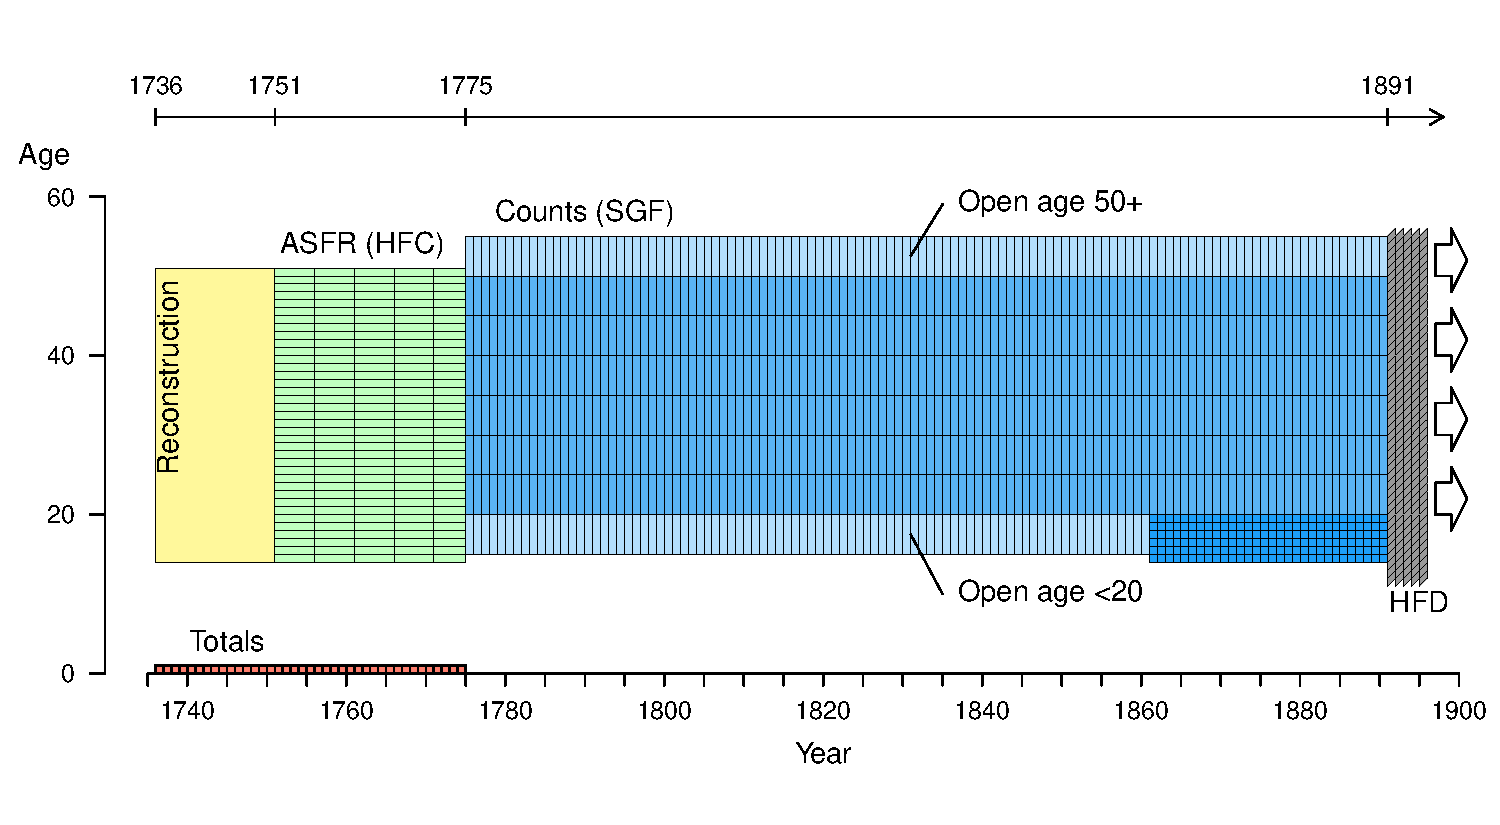
\includegraphics[scale=.65]{Figures/HistoricalDimensions.pdf}
\vspace{-2em}
\caption{Lexis diagram depiction of fertility data sources and discrete Lexis bins for the period 1736-1890. Total counts are used as constraints for years 1736-1750, denoted with red boxes at age 0. The yellow box from 1736 to 1750 denotes the Lexis region over which birth counts are reconstructed using indirect techniques. The blue boxes from 1775 to 1890 indicate various age-period bins of birth counts. Light blue indicates lower and upper open age groups. Dark blue boxes in ages 14-19 from 1861-1890 indicate single year age-period bins. The HFD provides single-year period-cohort bins for birth counts starting in 1891 (gray).}
\label{fig:histbins}
\end{center}
\end{figure}

\FloatBarrier
\subsection{Years 1736 - 1750}
\label{app:retroject}
Estimating birth counts by single year of age for the 15 year period from 1736 to 1750 requires several steps of data processing and some strong assumptions. First, we reverse-survive  females observed in the 1751 mid-year population census of Sweden, as extracted from the \citet{HMD} input database. Since this is a July 1 census, we take it as an acceptable proxy for exposure. The census originates in abridged ages $[0,1,3,5,10,15~...~90+]$. Examination of five year age groups suggests a underlying pattern age heaping, and for this reason we first smooth them using the so-called United Nations method \citep[see ][]{carrier1959reduction} as implemented in the \texttt{DemoTools} \texttt{R} package \citep{demotools}. We then graduate to single ages using the Sprague method \citep{sprague1880explanation,Shryock1973} as implemented in the \texttt{DemoTools} \texttt{R} package. This population is now the basis population to be reverse-survived through each single year until 1736, where we only make use of the fertile ages.

To reverse-survive, we use a standard survival curve defined as the age-specific arithmetic mean of the five single-age life table survival functions for the years 1751-1755 \citep{HMD}. The mid-year population count at age $x$, $n$ years before the 1751 census $P(x,1751-n)$ is estimated as:
		\begin{equation}
\label{eq:Pxhat}
P(x,1751-n) = P(x+n,1751) * \frac{\ell(x)}{\ell(x+n)} \tc
\end{equation}
where $\ell(x)$ is the standard survival function described.

The next step is to derive a standard ASFR curve, $F(x)$. ASFR for the years 1751-1775 is given by the \citet{HFC} in single ages and 5-year bins. If we rescale $F(x)$ in each 5-year period to sum to 1, one sees that there was very little shifting or shape changes in the period 1751-1774: each unity-scaled $F(x)$ curve is for practical purposes equivalent. We therefore take the standard fertility rate curve, $F^\star(x)$ to be their age-specific arithmetic mean, and we assume that it is valid for the year-range 1736 until 1750.

A first pass of unscaled birth counts at age $x$, $t$ years before 1751 is taken as the product of estimated exposure and $F^\star(x)$.
\begin{equation}
\widehat{B}^\star(x,1751-n) = P(x,1751-n) \cdot F^\star(x)
\end{equation}

The first pass of birth estimates implies a TFR of 1 in each year. Total births in each of these years $B(1751-n)$ is known \citep[][Tab.~27 \& Tab.~28]{sweden1969historisk}, so we derive our final estimate of age specific births, $\widehat{B}(x,1751-n)$ as:
		
		\begin{equation}
\widehat{B}(x,1751-n) = \widehat{B}^\star(x,1751-n) \cdot \frac{B(1751-n)}{\sum _{x=12}^{50}\widehat{B}^\star(x,1751-n) }
\end{equation}

At this stage of processing, birth count estimates for the years 1736-1750 are given in single ages (AP Lexis squares). Further adjustments are carried out in common with later periods and described in the following sections.

\subsection{Years 1751 - 1774}
\label{sec:hfc}
Estimating birth counts in single years and by single year of age for the 24 year period from 1751 to 1774 follows a similar logic, but it requires no retrojection. The \citet{HFC} provides ASFR in single ages\footnote{This data was graduated by the HFC from 5$\times$5 Lexis cells according to the HFC methods protocol \citep{grigorieva2015methods}.} in 5-year bins. The HMD provides exposure estimates $P(x,t)$ in single ages and years over this same period. A first-pass estimate of birth counts, $\widehat{B}(x,t)$ is given by:
		
		\begin{equation}
\widehat{B}(x,t) = P(x,t) \cdot F(x,t') \tc
				\end{equation}
				
				where $t'$ denotes the 5-year bin in which $t$ happens to fall. Year bins in the data are 5-years wide, and shifted up by 1, ergo 1751-1755, 1756-1760, and so forth. Following the convention of indexing to the lower bound, $t'$ is defined as:
				\begin{equation}
				t' = 5\floor{t/5}+1
				\end{equation}

Births by single year of mothers' age are then rescaled to sum to the annual totals reported in the HMD:
		\begin{equation}
		B(x,t) = \widehat{B}(x,t) * \frac{B(t)}{\sum _{x=12}^{50}\widehat{B}^(x,t)}
		\end{equation}
		
		At this stage of processing, birth count estimates for the years 1751-1774 are given in single ages (AP Lexis squares). Further adjustments are carried out in common with later periods and described in the following sections.
		
		\subsection{Years 1775 - 1890}
		\label{sec:sgf}
		Birth counts for the 116 year period from 1775 to 1890 are available from \citet{sgf1907}. These data are age-period classified, and given in a mixture of age classes, with a
		predominance 5-year age classes (especially for ages 20-50), but also sometimes
		single ages (especially for ages 15-19), and time-varying top and bottom open
		ages. We standardize these data in a few simple steps.
		
		First, births of unknown maternal age were redistributed proportionally to the distribution of births of known maternal age. Second, counts are graduated to single ages using the graduation method proposed by \citet{rizzi2015efficient} and implemented in \texttt{R} in the package \texttt{ungroup} \citep{ungroup}. 
		
		\subsection{Years 1736 - 1890}
		\label{sec:histadj}
		At this stage of processing all birth counts for years 1736 until 1890 are in single age-period (AP) bins, and datasets covering the three periods are merged into a common dataset. Two further adjustments are performed, the first to move AP-bins into period-cohort (PC) bins. The second adjustment compensates for the smoothness of graduation methods so as to preserve the expected relationship between a cohort's size its total offspring size.

\subsubsection{Adjustment to PC bins}
Counts were shifted from AP Lexis bins into PC bins assuming that half of the births in each single age $x$ bin go to the lower triangle of age $x+1$ and half to the upper triangle of the age-reached-during-the-year (PC) parallelogram at age $x$, as diagrammed in Fig.~\ref{fig:AP2PC}. At this point data are in a common format with the HFD data for the years 1891-2016, and these are merged into a single dataset.

\begin{figure}[ht!]
\centering
\begin{subfigure}{.3\textwidth}
\centering
\includegraphics[scale=.5]{Figures/App_split1.pdf}
\caption{AP square bins}
\label{fig:app1}
\end{subfigure}%
		\begin{subfigure}{.3\textwidth}
\centering
\includegraphics[scale=.5]{Figures/App_split2.pdf}
\caption{Split evenly to triangles}
\label{fig:app2}
\end{subfigure}
\begin{subfigure}{.3\textwidth}
\centering
\includegraphics[scale=.5]{Figures/App_split3.pdf}
\caption{Regroup to PC bins}
\label{fig:app3}
\end{subfigure}
\caption{The count regrouping procedure for years 1736 to 1890. Data are graduated to single ages (Fig.~\ref{fig:app1}), then split in half (Fig.~\ref{fig:app2}) and regrouped to period cohort (PC) bins (Fig.~\ref{fig:app3}).}
\label{fig:AP2PC}
\end{figure}

\FloatBarrier
\subsubsection{Cohort size adjustment}
\label{sec:cohadj}
At this stage of processing we have a harmonized dataset comprising a single series from 1736 until 2016 in consistent single-year PC bins. As such, one could produce the two time series represented in Fig.~\ref{fig:foldout}, albeit with a subtle artifact visible in Fig.~\ref{fig:toosmooth}. In area \textbf{A} of this figure, birth counts in age bins have been graduated using the previously mentioned pclm method, which has the usually-desired artifact of smoothness. For the affected range of years, mother cohorts are identified via the identity $C = P - A - 1$ .\footnote{One subtracts 1 because data are in period-cohort bins.} Since age patterns of counts are smooth, these sum in Lexis diagonals to a smooth time series of cohort total offspring, as seen in the profile of area \textbf{B} of the same figure. Area \textbf{C} of this figure delimits years 1875 until 1971, where both cohort and matched offspring sizes are directly observed, and where fluctuations would appear to co-vary quite strongly. For the sake of a more sensible count graduation and for reasons of aesthetic continuity, we have opted to adjust the counts in area \textbf{B} to carry the pattern of fluctuation observed over cohort size from 1736 to 1890.

\begin{figure}[ht!]
\centering
\includegraphics[scale=.6]{Figures/App_preAdjustment.pdf}
\caption{In reference years $\ge$ 1891 both births by year and cohort offspring are directly observed in single year bins, which means that the structural echo between total birth cohort and offspring size is preserved for reference years $\ge$ 1876  (\textbf{C}). Total per annum births in years $\le$ 1890 (\textbf{A}) are presumed accurate, and so first differences of these are observed. Offspring from cohorts born in years $\le$ 1876 (\textbf{B}) were partially (1836--1876) or entirely ($<$ 1836) born in years $\le$ 1890, implying a smooth redistribution over single years of mother cohorts. We wish to adjust the births in \textbf{B} to recuperate the kind of structural echo in \textbf{C}.}
\label{fig:toosmooth}
\end{figure}

This adjustment works by extracting the fluctuation pattern from \textbf{A} and transferring it to \textbf{B}. We do this by first smoothing the annual time series of total cohort size $B(t)$ according to some smoothness parameter, $\lambda$.\footnote{For the present case we've used a loess smoother, using the \texttt{R} function \texttt{loess()} with smoothing parameter $\lambda =$ \texttt{span}. It would be straightforward to swap this smoothing method out with a different one.} The ratio of $B(t)$ to the smoothed birth series $B(t)^s$ defines the multiplicative adjustment factor, $adj(t) = B(t)/B(t)^s$. Total offspring size $\mathbb{B}(c)$ is then adjusted as $\mathbb{B}(c)' = adj(t)*\mathbb{B}(c), \mathrm{~for~} c = t$. Counts in single ages are then rescaled to sum to the original totals in 5-year age groups, and counts for years $>$ 1890 are unaffected. The smoothing parameter is selected such that the linear relationship in fractional first differences $rd(B(t)) = \frac{B(t+1)-B(t)}{B(t)}$ between the annual birth series and adjusted offspring series $rd(\mathbb{B}(c)')$ for years 1736-1876 matches that for the reference years 1877-1971 as closely as possible. Specifically, we select $\lambda$ so as to minimize the sum of the difference in the slope and residual standard deviation for the periods before and after 1891. Further clarifications about this adjustment, and code for diagnostic plots can be found in the annotated code repository. The end effect is to adjust the series to look like Fig.~\ref{fig:better}.
					
					\begin{figure}[ht!]
					\centering
					\includegraphics[scale=.6]{Figures/App_postAdjustment.pdf}
					\caption{The adjusted birth series. Annual total births $B(t)$ on top axis and annual total offspring $\mathbb{B}(c)$ on bottom axis, with adjusted offspring counts $\mathbb{B}(c)'$ outlined.}
\label{fig:better}
\end{figure}
\end{appendix}

We adjusted in this way for the sake of a more nuanced time series of total offspring, but this approach may be used to good effect in graduating age-structured counts (births, deaths, populations) whenever time series are long enough to permit information on birth cohort size to propagate through the Lexis surface. These aspects are visible to some degree in the shaded polygons of Fig.~\ref{fig:foldout} in years $<$ 1891.

\subsection{Projected birth counts}
\label{sec:proj}
\todo{complete when exercise done}
Offspring counts by year of occurrence, $B(c,t)$ are only fully observed for years $\le$ 1971. To complete the reflection, we have opted to project birth counts for cohorts whose fertility careers are incomplete. This is done by combining a projection of cohort fertility rates using the method proposed by \citet{de1985time} with a standard projection of population denominators (mortality projection too? Could also just take the pop projection from Statistics Sweden.). The method used is parsimonious, and it performed very well in a comprehensive assessment of fertility forecast methods \citep{bohk2018forecast}. Light documentation to follow here, as well as an update of Fig.~\ref{fig:better}.

\subsection{Meandering baseline}
\label{sec:baseline}
A peculiar feature of Fig.~\ref{fig:foldout} is the meandering baseline, which replaces the standard straight-line $x$-axis. The baseline is derived from the crude cohort replacement rate $\mathbb{R}(c)$, defined as $\mathbb{R}(c) = \mathbb{B}(c=r) / B(t=r)$. This measure is not a replacement for the classic measure of net reproduction $R_0$, which differs in a few key ways: i) crude replacement is not sex-specific (our birth series is composed of boy and girl births combined), whereas $R_0$ is typically defined for females only. ii) while births arise from fertility rates over the life course, the number of potential mothers over the life course is not a mere function of mortality, but of migration as well, and the Swedish birth series will have been affected by heavy out-migration from 1850 until the Second World War, and some in-migration in more recent decades. Cohort $R_0$ is purged of population structure such as this (except to the extent that subgroups have differential vital rates), whereas $\mathbb{R}(c)$ is not, and for this reason we call it \emph{crude}.

The series of $\mathbb{R}(c)$ is rather smooth without further treatment, save for 11 periodic breaks between 1970 and 1840, a period of rupture between 1865 and 1880, and another set of at least four breaks since the great depression in the 1930s. Rather than preserve these ruptures, we opt to smooth them out and instead capture long term trends in $\mathbb{R}(c)$ in the baseline, as seen in Fig.~\ref{fig:meander}. Keeping the baseline meander smooth minimizes the visual penalty in assessing the variation in $\mathbb{B}(c)$ or $B(t)$ separately, and it enhances our ability to see the long term pattern. Specifically, we use use the \texttt{smooth.spline} from the \texttt{stats} \texttt{R} package, to smooth the $ln(\mathbb{R}(r))$ with smoothing parameter $\lambda = 0.00001$. The baseline that appears in Fig.~\ref{fig:refl} is the smooth prediction multiplied by 100,000.

\begin{figure}[ht!]
\centering
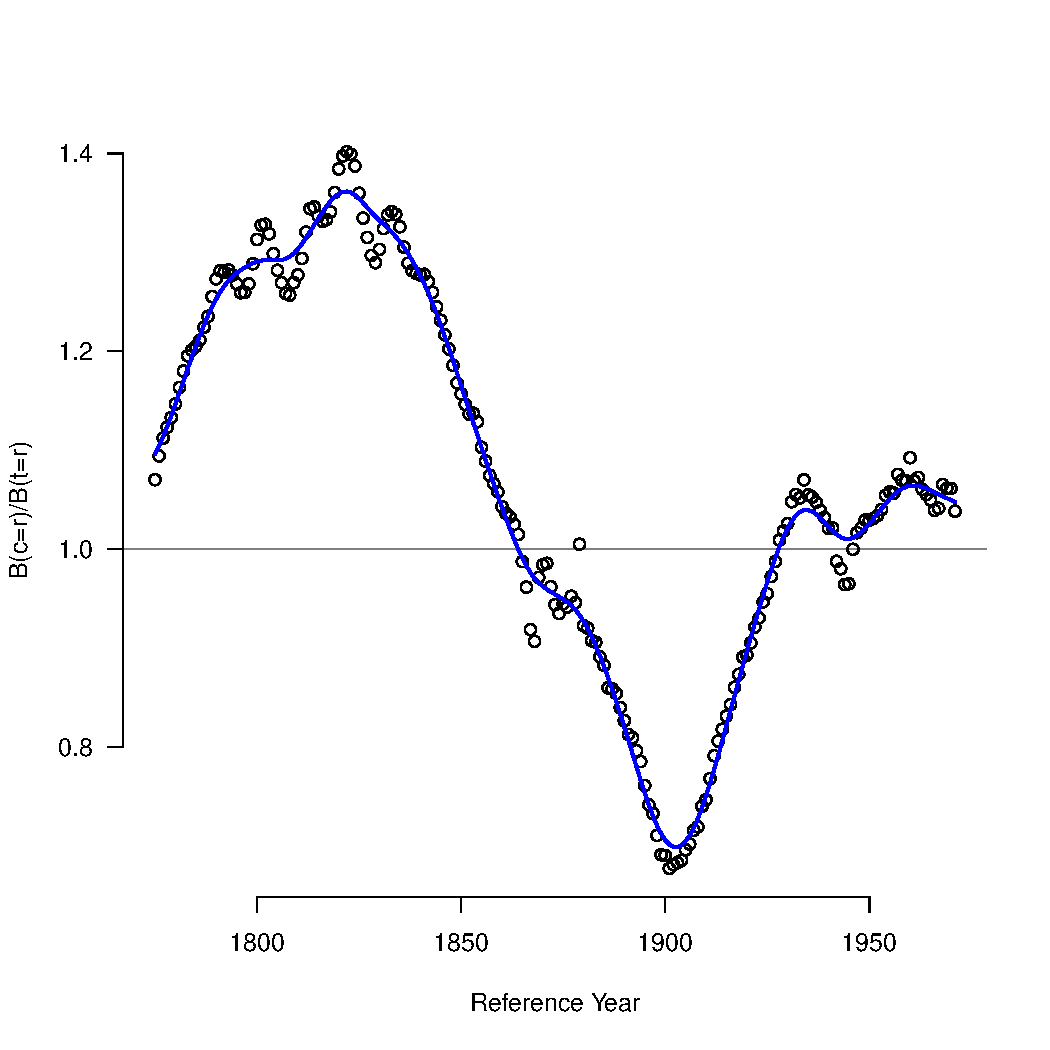
\includegraphics[scale=.6]{Figures/Meander.pdf}
\caption{The time series of crude cohort replacement, $\mathbb{R}(c)$, and its smooth pattern (blue line) on which the Fig.~\ref{fig:foldout} meandering baseline is based.}
\label{fig:meander}
\end{figure}




\end{appendix}
\pagebreak

\theendnotes
\pagebreak

\listoftables
\pagebreak

\listoffigures
\pagebreak
\bibliographystyle{plainnat}
  \bibliography{references} 
\end{document}

%\subsection{Notes on visual form}
%This visualization form derives from stacked area charts in general and river plots (theme river) and stream graphs in particular \citep{byron2008stacked}, but we wish to point out a few notable differences. Our birth flow visualization is composed of two separate stacked area graphs, where polygons appear in chronological order from left to right. If the top and bottom graph sections were vertically centered independently of one another, then these would comprise two ``river'' plots. Instead, the two series are squeezed together to share a $y$ coordinate at 0 on the baseline, and vertical centering is approximated on average by smooth baseline shifts as a function of the crude replacement ratio. 

%Different kinds of visual analytic tasks are probably penalized by this choice of form. For example, using the metrics proposed by \citet{thudt2016assessing}, we hypothesize that our visualization would perform poorly or moderately well in terms of ``individual discrimination'' because most birth distributions vary within the same order of magnitude. For example, it is not easy to visually discriminate the larger of ``number of children born in 1900 to mothers born between 1865 and 1869'' versus ``number of children that mothers born in 1900 had between the years 1925 and 1929'', (even though these share an $x$ coordinate) and such comparisons may be even more difficult the greater the distance in $y$ and $x$ between comparisons. 

%If we wish to compare the area of polygons, our reflected axes are advantageous: for example, it is not easy to visually compare the area of the top-level polygon ``children to mothers born 1870-1874'' versus the area of the bottom-level polygon ``children born 1910-1914''. The darkness and saturation of polygon fill colors transmit this information, but the two fill colors are too similar to be very helpful in this case, especially since they are non-adjacent. However, these two polygons are redundantly encoded in a more comparable way: the first is coded to the average from 1870-1874 of the total height on the bottom $y$ axis, and the second is encoded to the average total height from 1910-1914 on the top $y$ axis. This requires active decoding from the viewer, and such tasks are surely not quick, but likely result in precise judgments: Using height to decode, we see determine that the first polygon is larger than the second. For this kind of comparison, the polygons themselves are a distraction, as the same information is coded the height, but if there were no polygons then we would not be reminded that these two distributions are linked through time and through generations: the polygons overlap in $x$, and this is one of the prime data qualities that we wish to exemplify.

%Again using the metrics of \citet{thudt2016assessing}, we presume to fare \emph{very} well in terms of ``stream comparison'', since the rendering of each birth distribution is matched to $x$, and also \emph{very} well in terms of aggregate discrimination of top versus bottom (because the meandering baseline gives this). Our visualization would presumably perform moderately well in terms of aggregate discrimination of top plus bottom, because river and stream plots also performed well on this metric, and our visualization resembles these in its manner of centering. In our case, the stream centering method brings the crude replacement ratio to the fore. On the other hand, certain visual tasks are augmented due to the nature of the data: visual discrimination of polygons is all but guaranteed. Chronological order is clear to the viewer. Even so, we accept high losses of value look-up ability, for the sake of an aesthetic welcome mat to those who wish to learn more about the fundamentals of demography in general and the Swedish birth flow in particular. Few small questions can be answered with this graphic, but some large ones may be inspired.